% P2 -- The result: confidence is evidence-blind
\begin{frame}[t]{Result: confidence is evidence-blind}{The largest accuracy effect in \Etwo\ is invisible to confidence --- in every bin}
  \begin{columns}[T]
    \begin{column}{0.485\textwidth}
      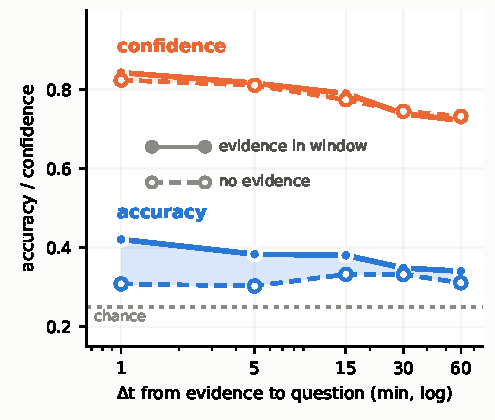
\includegraphics[width=\textwidth,height=0.72\textheight,keepaspectratio]{e2-ev-slide.pdf}
    \end{column}
    \begin{column}{0.495\textwidth}
      \vskip-0.3em
      {\scriptsize Token-matched, paired within each of \Nquestions\ questions:}
      \vskip0.35em
      \begin{center}\scriptsize\renewcommand{\arraystretch}{1.0}
        \begin{tabular}{@{}lcc@{}}
          \toprule
          \thead{\dt\ (min)} & \thead{\acc{$\Delta$accuracy} (pp)} & \thead{\conf{$\Delta$confidence} (pp)} \\
          \midrule
          \TabEtwoEvidenceByDt
          \bottomrule
        \end{tabular}
      \end{center}
      \vskip0.3em
      \claim{\scriptsize \acc{$\Delta$accuracy} runs \EtwoEvidenceSpread, excluding zero in \EtwoEvidenceAccSig\ bins --- the advantage decays as the cache saturates. \conf{$\Delta$confidence} spans zero in all \EtwoEvidenceBins\ and tracks neither the effect nor its decay.}
    \end{column}
  \end{columns}
\end{frame}
